\documentclass[25pt, portrait]{tikzposter}
\usepackage[utf8]{inputenc}


\geometry{paperwidth=80cm,paperheight=180cm}

\makeatletter
\setlength{\TP@visibletextwidth}{\textwidth-2\TP@innermargin}
\setlength{\TP@visibletextheight}{\textheight-2\TP@innermargin}

\def\title#1{\gdef\@title{\scalebox{\TP@titletextscale}{%
\begin{minipage}[t]{\linewidth}
\centering
#1
\par
\vspace{0.5em}
\end{minipage}%
}}}
\makeatother


\usepackage{etoolbox}
\makeatletter
\patchcmd{\TP@maketitle}
  {\Huge \sc}
  {\Huge}
  {}{}
\makeatother

\usepackage{mathrsfs} 
\usepackage{amssymb,amsmath,amsfonts}
\usepackage{capt-of}
\usepackage{grffile}
\usepackage{calc}
\usepackage{blindtext}
\usepackage{comment}

\newcommand*\mean[1]{\overline{#1}}


\renewcommand{\figurename}{Fig.}

\title{{\normalfont Diseño e implementación de un modelo de baja complejidad computacional para el pronóstico meteorológico en Colombia}}
\author{Randy S. Consuegra O. \\
\texttt{randyc@uninorte.edu.co}\\
Asesor: PhD. Elias Niño \\}
\institute{Departamento de Ingeniería de Sistemas y Computación\\
  Universidad del Norte}



\usetheme{Rays}


\tikzposterlatexaffectionproofoff

\begin{document}
\maketitle

\block{Introducción}
{
    Desde los inicios de las civilizaciones, ha sido de sumo interés el pronóstico meteorológico para, por ejemplo, actividades de vital importancia económica. \\
    En la actualidad, se ha logrado obtener modelos capaces de pronosticar hasta 72 horas, con baja incertidumbre, las condiciones meteorológicas del mundo en general. Dada la naturaleza caótica del estado del tiempo, su simulación mediante modelos matemáticos es computacionalmente costosa implicando el uso de servidores robustos con altos costos asociados. Por lo anterior, se plantea la necesidad de obtener un modelo matemático que nos permita realizar el pronóstico del clima, teniendo en cuenta componentes como la temperatura, la humedad, la presión y el viento, con baja incertidumbre y que admita retroalimentación. Este modelo debe ser de una complejidad computacional reducida, en comparación a los otros modelos y técnicas que se utilizan con la misma finalidad en la literatura. Además, estos resultados se deberán obtener al ejecutarse en máquinas de menor potencia (en comparación con los supercomputadores de instituciones y entidades privadas de Estados Unidos y Europa). 
}



\block{Metodología}
{
    En el texto de Chavarriaga [1] se presenta una metodología para proyectos de ingeniería de software con componente de investigación, y tomando elementos de esta metodología se desarrollará el proyecto.
    \begin{tikzfigure}
        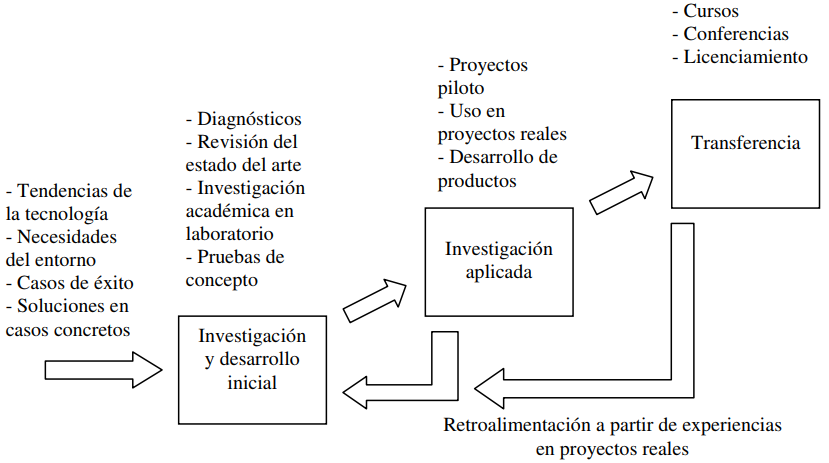
\includegraphics[width=0.6\textwidth]{images/metodologia.PNG}
    \end{tikzfigure}
    \captionof{figure}{Metodología propuesta en [1]}
}


\begin{columns}
    \column{0.5}
    \block{Solución}
    {
        La solución propuesta es realizar una solicitud mediante el protocolo FTP a los servidores de la National Oceanic and Atmospheric Administration (NOAA) para obtener los datos de los últimos 11 años, estos se ingresan al modelo, separándolos por cada hora en la que se realizó la muestra. Con los datos separados por hora, se aplica el modelo. Una vez obtenidos el pronostico, se validarán con los datos con la información del año presente, provista por la misma pagina.
        \begin{tikzfigure}
            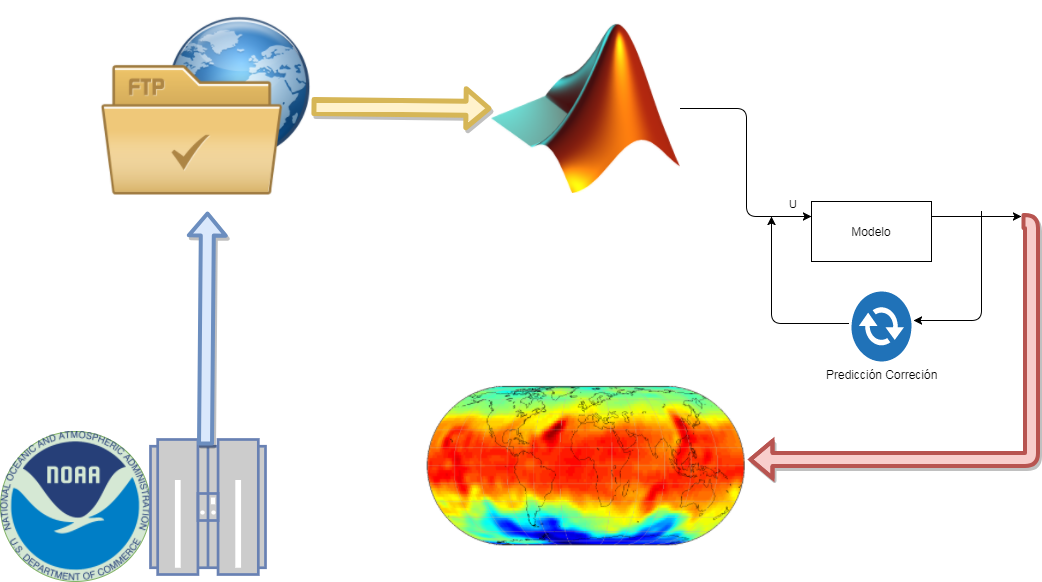
\includegraphics[width=0.4\textwidth]{images/diagram.png}
        \end{tikzfigure}
        \captionof{figure}{Esquema de la solución propuesta}
        El modelo parte del supuesto que todas las variables se pueden modelar con una distribución normal y que el error se propaga linealmente.
    }
    \column{0.5}
    \block{Modelo}
    {
        Se propone un modelo Markoviano de orden 1 para la realización del pronostico, tal como se presenta en el siguiente diagrama. 
        \begin{tikzfigure}
            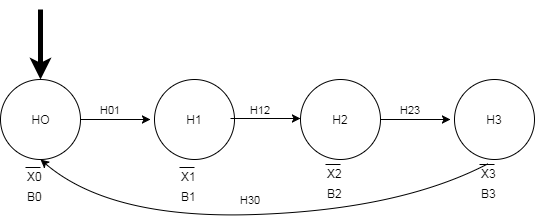
\includegraphics[width=0.4\textwidth]{images/Markovian.png}
        \end{tikzfigure}
        \captionof{figure}{Modelo propuesto}
        
        En el que $\mean{\mathbf{X}}_i \in \mathbb{R}^{n \times 1}$,$\mbox{H}_i$  es un vector de estados, $\mbox{H}_{i,i+1}$ es un vector de transición y $\mbox{B}_i$ es una matriz de covarianza en $\mathbb{R}^{n \times n}$. Luego:
        \begin{equation*} \label{eu_eqn}
            \mathcal P(x_{1}) \: \alpha \: \mathcal P(x_{01})\mathscr{L}(x_1|x_0)
        \end{equation*}
    
        \begin{equation*} 
            \mathscr{L}(x_1|x_0) \: \alpha \: {e}^{\frac{-1}{2}{\lVert x_0-G\cdot{x}_{01} \rVert}^2_{B_0^-1}}
        \end{equation*}
         Además, se propone: \\
         $G=[I \quad \boldsymbol{0}]  \in {R}^{n \times 2n}, \quad I,\boldsymbol{0} \in \mathbb{R}^{n \times n}$\\
        $Q=[\boldsymbol{0} \quad I]  \in {R}^{2n \times n}, \quad I,\boldsymbol{0} \in \mathbb{R}^{n \times n}$
    }
\end{columns}
\begin{columns}
    \column{0.5}
    \block{Distribución}
    {
        \begin{tikzfigure}
            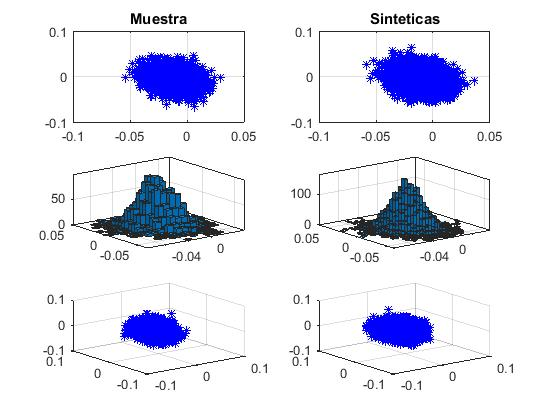
\includegraphics[width=0.4\textwidth]{images/probabilidad.jpg}
        \end{tikzfigure}
        \captionof{figure}{Distribución de probabilidad para $\Omega$ vs Variables sintéticas normalmente distribuidas.}
    }
    \column{0.5}
    \block{Resultados}
    {
        \begin{tikzfigure}
            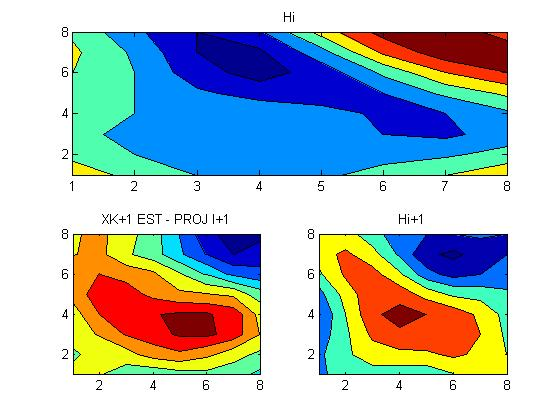
\includegraphics[width=0.4\textwidth]{images/untitled.jpg}
        \end{tikzfigure}
        \captionof{figure}{Pronostico de 6 horas, dado un estado inicial para $\Omega$.}
    }
\end{columns}

\begin{columns}
    \column{0.5}
    \block{Conclusiones y trabajos futuros}
    {
        A pesar que se descubrió que las variables en su mayoría no estaban normalmente distribuidas, el modelo es capaz de realizar pronósticos de 6 horas para una variable dada con excelente precisión y con menor consumo de procesamiento en la maquina, en especial cuando están normalmente distribuidas. Se deja para próximos trabajos implementar una mezcla gaussiana para poder realizar el pronostico en caso más general. 
    }
    \column{0.5}
    \block{Referencias}
    {
        \renewcommand{\section}[2]{}%
        \begin{thebibliography}{}
        
        \bibitem  J. A. Chavarriaga, L. Hugo, and F. Arboleda, “Modelo de Investigación en Ingeniería del Software: Una propuesta de investigación tecnológica.”
        \bibitem  P. Lynch, “The origins of computer weather prediction and climate modeling,” J. Comput. Phys., vol. 227, no. 7, pp. 3431–3444, Mar. 2008.
        \bibitem  S. Khajure and S. W. Mohod, “Future Weather Forecasting Using Soft Computing Techniques,” Procedia Comput. Sci., vol. 78, pp. 402–407, 2016.
        \end{thebibliography}
    }
\end{columns}

\node [above right,
       outer sep=0pt,
       minimum width=20cm,
       minimum height=7cm,
       align=center,font=\Huge,] at (bottomleft) {
\includegraphics{images/uninorte.png}};

\end{document}
